\documentclass{article}
\usepackage{graphicx} % Required for inserting images
\usepackage{amsmath}
\usepackage{tikz}
\usepackage{amssymb}
\usetikzlibrary{positioning,calc}
\usepackage[margin=1in]{geometry}
\title{Path Planners}
\author{Neal Ramaswamy}
\date{July 2025}
\begin{document}
\maketitle
\section{Introduction}
\section{Dijkstra's Algorithm}
\subsection{Basic Steps}
\begin{enumerate}
    \item Set source vertex distances $d_s$ = 0; for all other vertices' $d_v$ = $\infty$
    \item Push the source vertex into a min-priority queue with its distance ($V_s$, $d_s$)
    \item Algorithm Loop starts
        \begin{enumerate}
            \item Pop the min vertex $V_{\text{min}}$, $d_{\text{min}}$ from the queue
            \item For each connected vertex $V$
                \begin{enumerate}
                    \item Calculate the distance $d$ of the edge $V -> V_{\text{min}}$
                    \item Set $d = min(d + d_{\text{min}}, d_v)$ and set $d_v = d$
                    \item Push to the queue ($V$, $d$)
                    
                \end{enumerate}
        \end{enumerate}
    \item Repeat Algorithm Loop until Queue is empty
\end{enumerate}

\section{Dijkstra's Algorithm}

\subsection{Overview}
Dijkstra's algorithm finds the shortest path from a source vertex to all other vertices in a weighted graph with non-negative edge weights.

\subsection{Algorithm}
\textbf{Input:} A weighted directed graph $G = (V, E)$ with weight function $w: E \to \mathbb{R}_{\geq 0}$ and source vertex $s \in V$.

\textbf{Output:} Distance array $d$ where $d[v]$ represents the shortest distance from $s$ to vertex $v$.

\textbf{Initialization:}
\begin{enumerate}
    \item Set $d[s] = 0$ and $d[v] = \infty$ for all $v \in V \setminus \{s\}$
    \item Create a min-priority queue $Q$ and insert $(s, 0)$
    \item Mark all vertices as unvisited
\end{enumerate}

\textbf{Main Loop:}
\begin{enumerate}
    \item While $Q$ is not empty:
    \begin{enumerate}
        \item Extract $(u, d_u) = \text{ExtractMin}(Q)$
        \item If $u$ has been visited, continue to next iteration
        \item Mark $u$ as visited
        \item For each neighbor $v$ of $u$ where $(u,v) \in E$:
        \begin{enumerate}
            \item Calculate tentative distance: $d_{\text{new}} = d[u] + w(u,v)$
            \item If $d_{\text{new}} < d[v]$:
            \begin{itemize}
                \item Update $d[v] = d_{\text{new}}$
                \item Insert $(v, d_{\text{new}})$ into $Q$
            \end{itemize}
        \end{enumerate}
    \end{enumerate}
\end{enumerate}

\subsection{Correctness}
The algorithm maintains the invariant that when a vertex is marked as visited, $d[v]$ contains the shortest distance from $s$ to $v$.

\subsection{Complexity}
\textbf{Time:} $O((|V| + |E|) \log |V|)$ using a binary heap\\
\textbf{Space:} $O(|V|)$

\subsection{Algorithm Requirements}
\begin{enumerate}
    \item Non-negative edge weights
\end{enumerate}

\subsection{Simple Example}
% PICTURE 1
\begin{center}
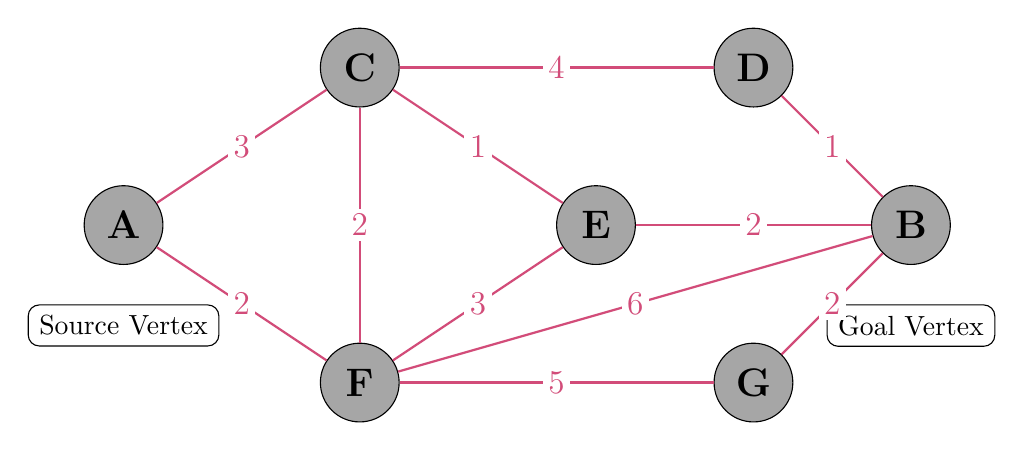
\begin{tikzpicture}[
    node distance=3cm,
    vertex/.style={circle, draw, fill=gray!70, minimum size=1cm, font=\Large\bfseries},
    edge/.style={draw, thick, color=purple!70},
    weight/.style={fill=white, inner sep=2pt, font=\large}
]

% Define node positions
\node[vertex] (A) at (-4, 0) {A};
\node[vertex] (C) at (-1, 2) {C};
\node[vertex] (F) at (-1, -2) {F};
\node[vertex] (E) at (2, 0) {E};
\node[vertex] (D) at (4, 2) {D};
\node[vertex] (B) at (6, 0) {B};
\node[vertex] (G) at (4, -2) {G};

% Add source vertex label
\node[below=0.5cm of A, draw, fill=white, rounded corners, inner sep=4pt] {Source Vertex};

% Add goal vertex label
\node[below=0.5cm of B, draw, fill=white, rounded corners, inner sep=4pt] {Goal Vertex};

% Draw edges with weights
\draw[edge] (A) -- (C) node[weight, midway] {3};
\draw[edge] (A) -- (F) node[weight, midway] {2};
\draw[edge] (C) -- (D) node[weight, midway] {4};
\draw[edge] (C) -- (E) node[weight, midway] {1};
\draw[edge] (C) -- (F) node[weight, midway] {2};
\draw[edge] (E) -- (F) node[weight, midway] {3};
\draw[edge] (E) -- (B) node[weight, midway] {2};
\draw[edge] (F) -- (B) node[weight, midway] {6};
\draw[edge] (D) -- (B) node[weight, midway] {1};
\draw[edge] (B) -- (G) node[weight, midway] {2};
\draw[edge] (F) -- (G) node[weight, midway] {5};

\end{tikzpicture}
\end{center}
% ----------- PICTURE 2 ----------
\subsection{Algorithm Initialization}
\begin{center}
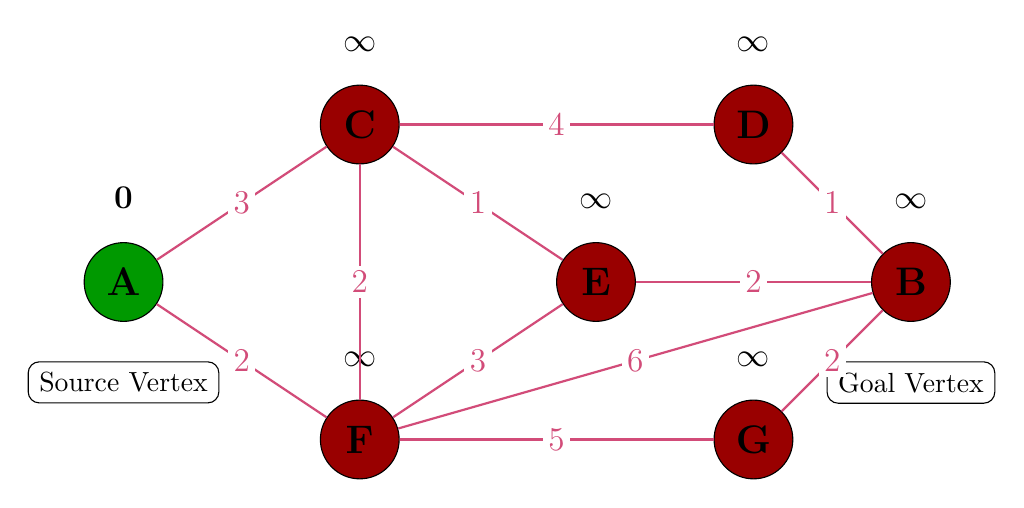
\begin{tikzpicture}[
    node distance=3cm,
    vertex/.style={circle, draw, fill=gray!70, minimum size=1cm, font=\Large\bfseries},
    edge/.style={draw, thick, color=purple!70},
    weight/.style={fill=white, inner sep=2pt, font=\large}
]

% Define node positions
\node[vertex, fill=green!60!black] (A) at (-4, 0) {A};
\node[vertex, fill=red!60!black] (C) at (-1, 2) {C};
\node[vertex, fill=red!60!black] (F) at (-1, -2) {F};
\node[vertex, fill=red!60!black] (E) at (2, 0) {E};
\node[vertex, fill=red!60!black] (D) at (4, 2) {D};
\node[vertex, fill=red!60!black] (B) at (6, 0) {B};
\node[vertex, fill=red!60!black] (G) at (4, -2) {G};

% Add distance labels above vertices
\node[above=0.3cm of A, font=\large\bfseries] {0};
\node[above=0.3cm of C, font=\large\bfseries] {$\infty$};
\node[above=0.3cm of F, font=\large\bfseries] {$\infty$};
\node[above=0.3cm of E, font=\large\bfseries] {$\infty$};
\node[above=0.3cm of D, font=\large\bfseries] {$\infty$};
\node[above=0.3cm of B, font=\large\bfseries] {$\infty$};
\node[above=0.3cm of G, font=\large\bfseries] {$\infty$};

% Add source vertex label
\node[below=0.5cm of A, draw, fill=white, rounded corners, inner sep=4pt] {Source Vertex};

% Add goal vertex label
\node[below=0.5cm of B, draw, fill=white, rounded corners, inner sep=4pt] {Goal Vertex};

% Draw edges with weights
\draw[edge] (A) -- (C) node[weight, midway] {3};
\draw[edge] (A) -- (F) node[weight, midway] {2};
\draw[edge] (C) -- (D) node[weight, midway] {4};
\draw[edge] (C) -- (E) node[weight, midway] {1};
\draw[edge] (C) -- (F) node[weight, midway] {2};
\draw[edge] (E) -- (F) node[weight, midway] {3};
\draw[edge] (E) -- (B) node[weight, midway] {2};
\draw[edge] (F) -- (B) node[weight, midway] {6};
\draw[edge] (D) -- (B) node[weight, midway] {1};
\draw[edge] (B) -- (G) node[weight, midway] {2};
\draw[edge] (F) -- (G) node[weight, midway] {5};

\end{tikzpicture}
\end{center}

% ----------- PICTURE 3 ----------
\subsection{Processing Source Vertex A}
\begin{center}
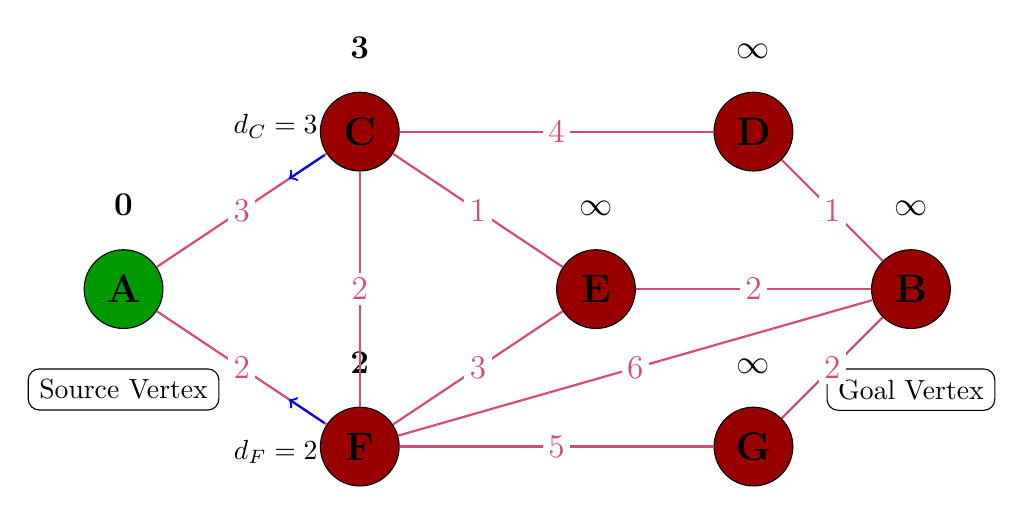
\begin{tikzpicture}[
    node distance=3cm,
    vertex/.style={circle, draw, fill=gray!70, minimum size=1cm, font=\Large\bfseries},
    edge/.style={draw, thick, color=purple!70},
    weight/.style={fill=white, inner sep=2pt, font=\large}
]

% Define node positions
\node[vertex, fill=green!60!black] (A) at (-4, 0) {A};
\node[vertex, fill=red!60!black] (C) at (-1, 2) {C};
\node[vertex, fill=red!60!black] (F) at (-1, -2) {F};
\node[vertex, fill=red!60!black] (E) at (2, 0) {E};
\node[vertex, fill=red!60!black] (D) at (4, 2) {D};
\node[vertex, fill=red!60!black] (B) at (6, 0) {B};
\node[vertex, fill=red!60!black] (G) at (4, -2) {G};

% Add distance labels above vertices
\node[above=0.3cm of A, font=\large\bfseries] {0};
\node[above=0.3cm of C, font=\large\bfseries] {3};
\node[above=0.3cm of F, font=\large\bfseries] {2};
\node[above=0.3cm of E, font=\large\bfseries] {$\infty$};
\node[above=0.3cm of D, font=\large\bfseries] {$\infty$};
\node[above=0.3cm of B, font=\large\bfseries] {$\infty$};
\node[above=0.3cm of G, font=\large\bfseries] {$\infty$};

% Add source vertex label
\node[below=0.5cm of A, draw, fill=white, rounded corners, inner sep=4pt] {Source Vertex};

% Add goal vertex label
\node[below=0.5cm of B, draw, fill=white, rounded corners, inner sep=4pt] {Goal Vertex};

% Draw edges with weights
\draw[edge] (A) -- (C) node[weight, midway] {3} node[pos=0.7, above=5mm, color=black] {$d_C = 3$};
\draw[edge] (A) -- (F) node[weight, midway] {2} node[pos=0.7, below=5mm, color=black] {$d_F = 2$};
\draw[edge] (C) -- (D) node[weight, midway] {4};
\draw[edge] (C) -- (E) node[weight, midway] {1};
\draw[edge] (C) -- (F) node[weight, midway] {2};
\draw[edge] (E) -- (F) node[weight, midway] {3};
\draw[edge] (E) -- (B) node[weight, midway] {2};
\draw[edge] (F) -- (B) node[weight, midway] {6};
\draw[edge] (D) -- (B) node[weight, midway] {1};
\draw[edge] (B) -- (G) node[weight, midway] {2};
\draw[edge] (F) -- (G) node[weight, midway] {5};

% Blue arrows for Picture 3 (pointing from child to parent)
\draw[->, blue, thick] ($ (C)!0.15!(A) $) -- ($ (C)!0.3!(A) $);
\draw[->, blue, thick] ($ (F)!0.15!(A) $) -- ($ (F)!0.3!(A) $);

\end{tikzpicture}
\end{center}

% ----------- PICTURE 4 ----------
\subsection{Processing Vertex F}
\begin{center}
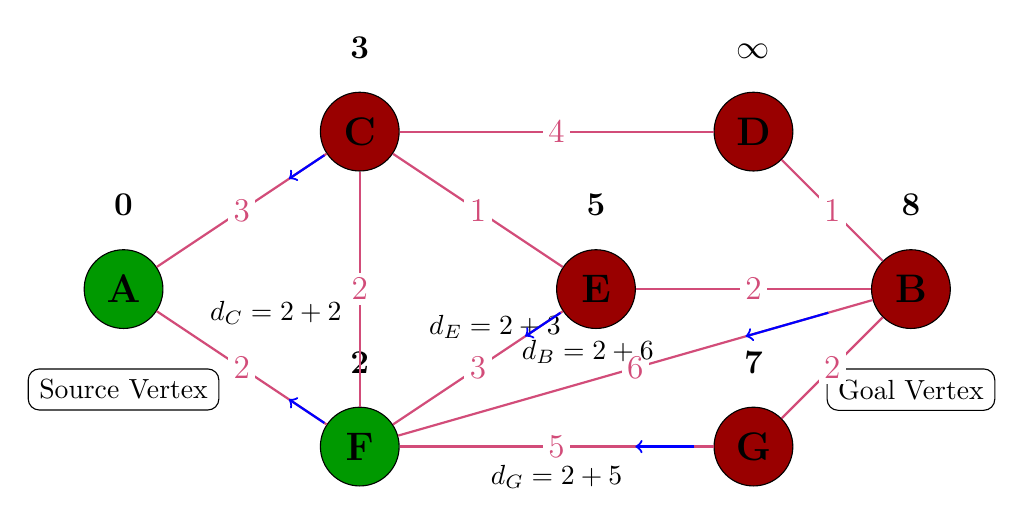
\begin{tikzpicture}[
    node distance=3cm,
    vertex/.style={circle, draw, fill=gray!70, minimum size=1cm, font=\Large\bfseries},
    edge/.style={draw, thick, color=purple!70},
    weight/.style={fill=white, inner sep=2pt, font=\large}
]

% Define node positions
\node[vertex, fill=green!60!black] (A) at (-4, 0) {A};
\node[vertex, fill=red!60!black] (C) at (-1, 2) {C};
\node[vertex, fill=green!60!black] (F) at (-1, -2) {F};
\node[vertex, fill=red!60!black] (E) at (2, 0) {E};
\node[vertex, fill=red!60!black] (D) at (4, 2) {D};
\node[vertex, fill=red!60!black] (B) at (6, 0) {B};
\node[vertex, fill=red!60!black] (G) at (4, -2) {G};

% Add distance labels above vertices
\node[above=0.3cm of A, font=\large\bfseries] {0};
\node[above=0.3cm of C, font=\large\bfseries] {3};
\node[above=0.3cm of F, font=\large\bfseries] {2};
\node[above=0.3cm of E, font=\large\bfseries] {5};
\node[above=0.3cm of D, font=\large\bfseries] {$\infty$};
\node[above=0.3cm of B, font=\large\bfseries] {8};
\node[above=0.3cm of G, font=\large\bfseries] {7};

% Add source vertex label
\node[below=0.5cm of A, draw, fill=white, rounded corners, inner sep=4pt] {Source Vertex};

% Add goal vertex label
\node[below=0.5cm of B, draw, fill=white, rounded corners, inner sep=4pt] {Goal Vertex};

% Draw edges with weights and distance calculations
\draw[edge] (A) -- (C) node[weight, midway] {3};
\draw[edge] (A) -- (F) node[weight, midway] {2};
\draw[edge] (C) -- (D) node[weight, midway] {4};
\draw[edge] (C) -- (E) node[weight, midway] {1};
\draw[edge] (C) -- (F) node[weight, midway] {2} node[pos=0.6, left=1mm, color=black] {$d_C = 2 + 2$};
\draw[edge] (E) -- (F) node[weight, midway] {3} node[pos=0.4, above=1mm, color=black] {$d_E = 2 + 3$};
\draw[edge] (E) -- (B) node[weight, midway] {2};
\draw[edge] (F) -- (B) node[weight, midway] {6} node[pos=0.4, above=1mm, color=black] {$d_B = 2 + 6$};
\draw[edge] (D) -- (B) node[weight, midway] {1};
\draw[edge] (B) -- (G) node[weight, midway] {2};
\draw[edge] (F) -- (G) node[weight, midway] {5} node[pos=0.5, below=1mm, color=black] {$d_G = 2 + 5$};

% Blue arrows for Picture 4 (pointing from child to parent)
\draw[->, blue, thick] ($ (E)!0.15!(F) $) -- ($ (E)!0.3!(F) $);
\draw[->, blue, thick] ($ (B)!0.15!(F) $) -- ($ (B)!0.3!(F) $);
\draw[->, blue, thick] ($ (G)!0.15!(F) $) -- ($ (G)!0.3!(F) $);
\draw[->, blue, thick] ($ (C)!0.15!(A) $) -- ($ (C)!0.3!(A) $);
\draw[->, blue, thick] ($ (F)!0.15!(A) $) -- ($ (F)!0.3!(A) $);

\end{tikzpicture}
\end{center}

% ----------- PICTURE 5 ----------
\subsection{Processing Vertex C}
\begin{center}
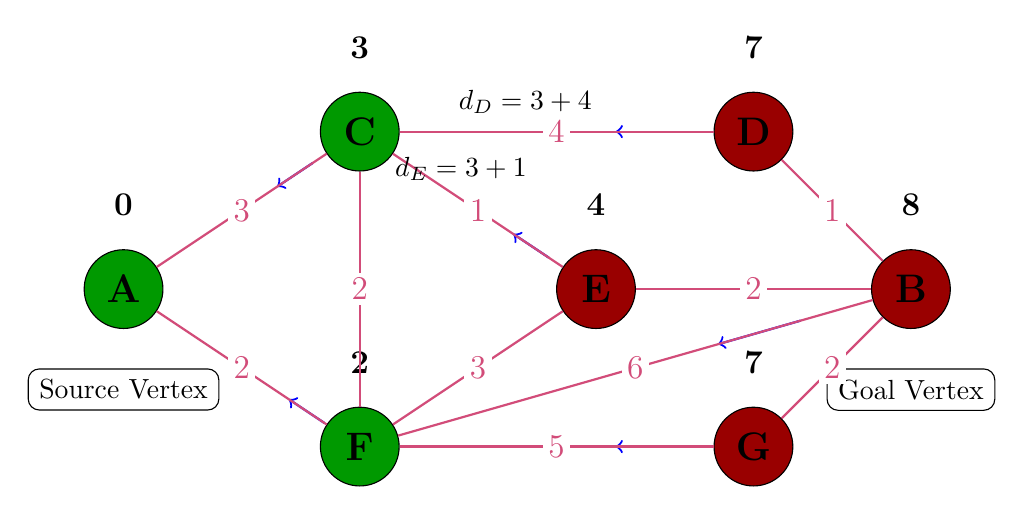
\begin{tikzpicture}[
    node distance=3cm,
    vertex/.style={circle, draw, fill=gray!70, minimum size=1cm, font=\Large\bfseries},
    edge/.style={draw, thick, color=purple!70},
    weight/.style={fill=white, inner sep=2pt, font=\large}
]

% Define node positions
\node[vertex, fill=green!60!black] (A) at (-4, 0) {A};
\node[vertex, fill=green!60!black] (C) at (-1, 2) {C};
\node[vertex, fill=green!60!black] (F) at (-1, -2) {F};
\node[vertex, fill=red!60!black] (E) at (2, 0) {E};
\node[vertex, fill=red!60!black] (D) at (4, 2) {D};
\node[vertex, fill=red!60!black] (B) at (6, 0) {B};
\node[vertex, fill=red!60!black] (G) at (4, -2) {G};

% Blue arrows for Picture 5 (pointing from child to parent)
\draw[->, blue, thick] ($ (E)!0.2!(C) $) -- ($ (E)!0.35!(C) $);
\draw[->, blue, thick] ($ (D)!0.2!(C) $) -- ($ (D)!0.35!(C) $);
\draw[->, blue, thick] ($ (B)!0.2!(F) $) -- ($ (B)!0.35!(F) $);
\draw[->, blue, thick] ($ (G)!0.2!(F) $) -- ($ (G)!0.35!(F) $);
\draw[->, blue, thick] ($ (C)!0.2!(A) $) -- ($ (C)!0.35!(A) $);
\draw[->, blue, thick] ($ (F)!0.15!(A) $) -- ($ (F)!0.3!(A) $);

% Add distance labels above vertices
\node[above=0.3cm of A, font=\large\bfseries] {0};
\node[above=0.3cm of C, font=\large\bfseries] {3};
\node[above=0.3cm of F, font=\large\bfseries] {2};
\node[above=0.3cm of E, font=\large\bfseries] {4};
\node[above=0.3cm of D, font=\large\bfseries] {7};
\node[above=0.3cm of B, font=\large\bfseries] {8};
\node[above=0.3cm of G, font=\large\bfseries] {7};

% Add source vertex label
\node[below=0.5cm of A, draw, fill=white, rounded corners, inner sep=4pt] {Source Vertex};

% Add goal vertex label
\node[below=0.5cm of B, draw, fill=white, rounded corners, inner sep=4pt] {Goal Vertex};

% Draw edges with weights and distance calculations
\draw[edge] (A) -- (C) node[weight, midway] {3};
\draw[edge] (A) -- (F) node[weight, midway] {2};
\draw[edge] (C) -- (D) node[weight, midway] {4} node[pos=0.4, above=1mm, color=black] {$d_D = 3 + 4$};
\draw[edge] (C) -- (E) node[weight, midway] {1} node[pos=0.4, above=1mm, color=black] {$d_E = 3 + 1$};
\draw[edge] (C) -- (F) node[weight, midway] {2};
\draw[edge] (E) -- (F) node[weight, midway] {3};
\draw[edge] (E) -- (B) node[weight, midway] {2};
\draw[edge] (F) -- (B) node[weight, midway] {6};
\draw[edge] (D) -- (B) node[weight, midway] {1};
\draw[edge] (B) -- (G) node[weight, midway] {2};
\draw[edge] (F) -- (G) node[weight, midway] {5};

\end{tikzpicture}
\end{center}

% ----------- PICTURE 6 ----------
\subsection{Processing Vertex E}
\begin{center}
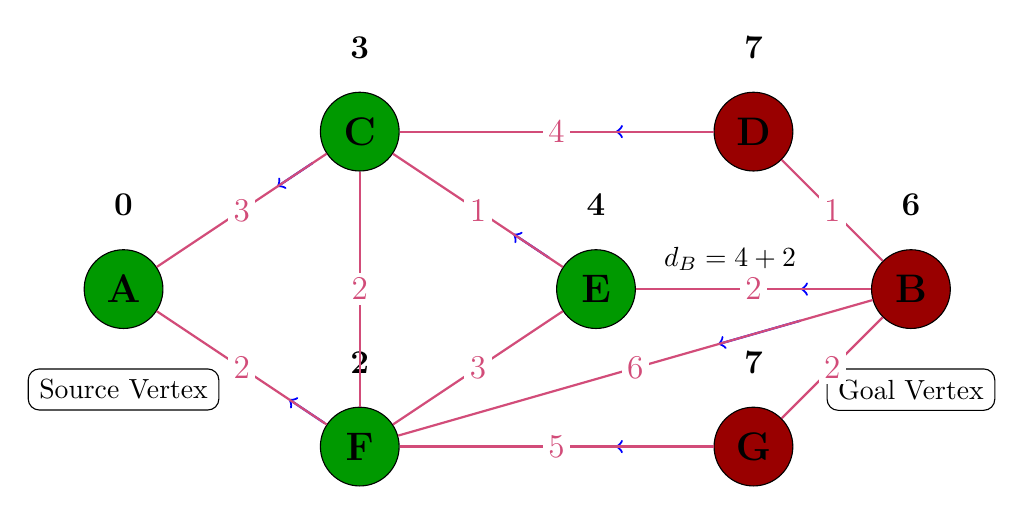
\begin{tikzpicture}[
    node distance=3cm,
    vertex/.style={circle, draw, fill=gray!70, minimum size=1cm, font=\Large\bfseries},
    edge/.style={draw, thick, color=purple!70},
    weight/.style={fill=white, inner sep=2pt, font=\large}
]

% Define node positions
\node[vertex, fill=green!60!black] (A) at (-4, 0) {A};
\node[vertex, fill=green!60!black] (C) at (-1, 2) {C};
\node[vertex, fill=green!60!black] (F) at (-1, -2) {F};
\node[vertex, fill=green!60!black] (E) at (2, 0) {E};
\node[vertex, fill=red!60!black] (D) at (4, 2) {D};
\node[vertex, fill=red!60!black] (B) at (6, 0) {B};
\node[vertex, fill=red!60!black] (G) at (4, -2) {G};

% Blue arrows for Picture 6 (pointing from child to parent)
\draw[->, blue, thick] ($ (D)!0.2!(C) $) -- ($ (D)!0.35!(C) $);
\draw[->, blue, thick] ($ (B)!0.2!(E) $) -- ($ (B)!0.35!(E) $);
\draw[->, blue, thick] ($ (G)!0.2!(F) $) -- ($ (G)!0.35!(F) $);
\draw[->, blue, thick] ($ (C)!0.2!(A) $) -- ($ (C)!0.35!(A) $);
\draw[->, blue, thick] ($ (E)!0.2!(C) $) -- ($ (E)!0.35!(C) $);
\draw[->, blue, thick] ($ (F)!0.15!(A) $) -- ($ (F)!0.3!(A) $);
\draw[->, blue, thick] ($ (B)!0.2!(F) $) -- ($ (B)!0.35!(F) $);

% Add distance labels above vertices
\node[above=0.3cm of A, font=\large\bfseries] {0};
\node[above=0.3cm of C, font=\large\bfseries] {3};
\node[above=0.3cm of F, font=\large\bfseries] {2};
\node[above=0.3cm of E, font=\large\bfseries] {4};
\node[above=0.3cm of D, font=\large\bfseries] {7};
\node[above=0.3cm of B, font=\large\bfseries] {6};
\node[above=0.3cm of G, font=\large\bfseries] {7};

% Add source vertex label
\node[below=0.5cm of A, draw, fill=white, rounded corners, inner sep=4pt] {Source Vertex};

% Add goal vertex label
\node[below=0.5cm of B, draw, fill=white, rounded corners, inner sep=4pt] {Goal Vertex};

% Draw edges with weights and distance calculations
\draw[edge] (A) -- (C) node[weight, midway] {3};
\draw[edge] (A) -- (F) node[weight, midway] {2};
\draw[edge] (C) -- (D) node[weight, midway] {4};
\draw[edge] (C) -- (E) node[weight, midway] {1};
\draw[edge] (C) -- (F) node[weight, midway] {2};
\draw[edge] (E) -- (F) node[weight, midway] {3};
\draw[edge] (E) -- (B) node[weight, midway] {2} node[pos=0.4, above=1mm, color=black] {$d_B = 4 + 2$};
\draw[edge] (F) -- (B) node[weight, midway] {6};
\draw[edge] (D) -- (B) node[weight, midway] {1};
\draw[edge] (B) -- (G) node[weight, midway] {2};
\draw[edge] (F) -- (G) node[weight, midway] {5};

\end{tikzpicture}
\end{center}

% ----------- PICTURE 7 ----------
\subsection{Processing Vertex B}
\begin{center}
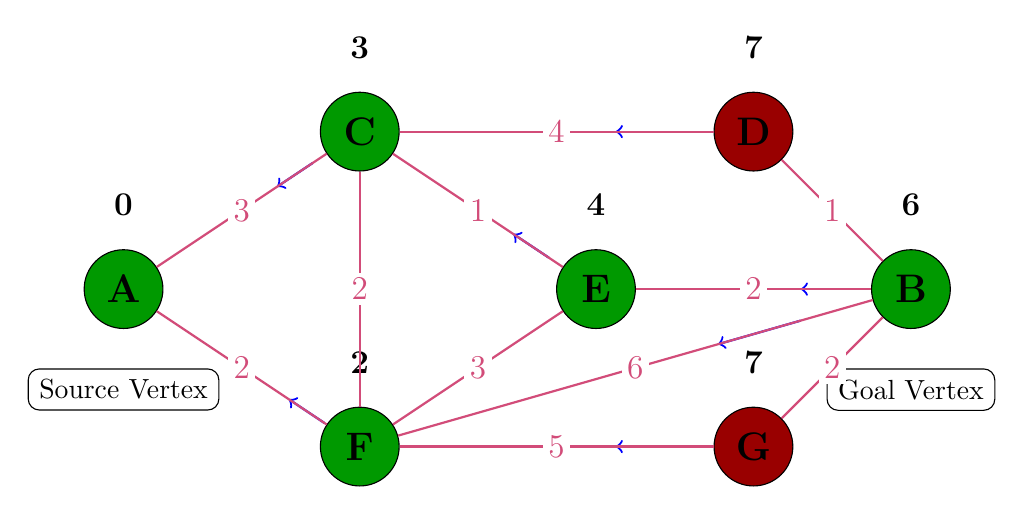
\begin{tikzpicture}[
    node distance=3cm,
    vertex/.style={circle, draw, fill=gray!70, minimum size=1cm, font=\Large\bfseries},
    edge/.style={draw, thick, color=purple!70},
    weight/.style={fill=white, inner sep=2pt, font=\large}
]

% Define node positions
\node[vertex, fill=green!60!black] (A) at (-4, 0) {A};
\node[vertex, fill=green!60!black] (C) at (-1, 2) {C};
\node[vertex, fill=green!60!black] (F) at (-1, -2) {F};
\node[vertex, fill=green!60!black] (E) at (2, 0) {E};
\node[vertex, fill=red!60!black] (D) at (4, 2) {D};
\node[vertex, fill=green!60!black] (B) at (6, 0) {B};
\node[vertex, fill=red!60!black] (G) at (4, -2) {G};

% Blue arrows for Picture 7 (pointing from child to parent)
\draw[->, blue, thick] ($ (D)!0.2!(C) $) -- ($ (D)!0.35!(C) $);
\draw[->, blue, thick] ($ (G)!0.2!(F) $) -- ($ (G)!0.35!(F) $);
\draw[->, blue, thick] ($ (C)!0.2!(A) $) -- ($ (C)!0.35!(A) $);
\draw[->, blue, thick] ($ (E)!0.2!(C) $) -- ($ (E)!0.35!(C) $);
\draw[->, blue, thick] ($ (B)!0.2!(E) $) -- ($ (B)!0.35!(E) $);
\draw[->, blue, thick] ($ (F)!0.15!(A) $) -- ($ (F)!0.3!(A) $);
\draw[->, blue, thick] ($ (B)!0.2!(F) $) -- ($ (B)!0.35!(F) $);

% Add distance labels above vertices
\node[above=0.3cm of A, font=\large\bfseries] {0};
\node[above=0.3cm of C, font=\large\bfseries] {3};
\node[above=0.3cm of F, font=\large\bfseries] {2};
\node[above=0.3cm of E, font=\large\bfseries] {4};
\node[above=0.3cm of D, font=\large\bfseries] {7};
\node[above=0.3cm of B, font=\large\bfseries] {6};
\node[above=0.3cm of G, font=\large\bfseries] {7};

% Add source vertex label
\node[below=0.5cm of A, draw, fill=white, rounded corners, inner sep=4pt] {Source Vertex};

% Add goal vertex label
\node[below=0.5cm of B, draw, fill=white, rounded corners, inner sep=4pt] {Goal Vertex};

% Draw edges with weights
\draw[edge] (A) -- (C) node[weight, midway] {3};
\draw[edge] (A) -- (F) node[weight, midway] {2};
\draw[edge] (C) -- (D) node[weight, midway] {4};
\draw[edge] (C) -- (E) node[weight, midway] {1};
\draw[edge] (C) -- (F) node[weight, midway] {2};
\draw[edge] (E) -- (F) node[weight, midway] {3};
\draw[edge] (E) -- (B) node[weight, midway] {2};
\draw[edge] (F) -- (B) node[weight, midway] {6};
\draw[edge] (D) -- (B) node[weight, midway] {1};
\draw[edge] (B) -- (G) node[weight, midway] {2};
\draw[edge] (F) -- (G) node[weight, midway] {5};

\end{tikzpicture}
\end{center}

% ----------- PICTURE 8 ----------
\subsection{Shortest Path from B to A}
\begin{center}
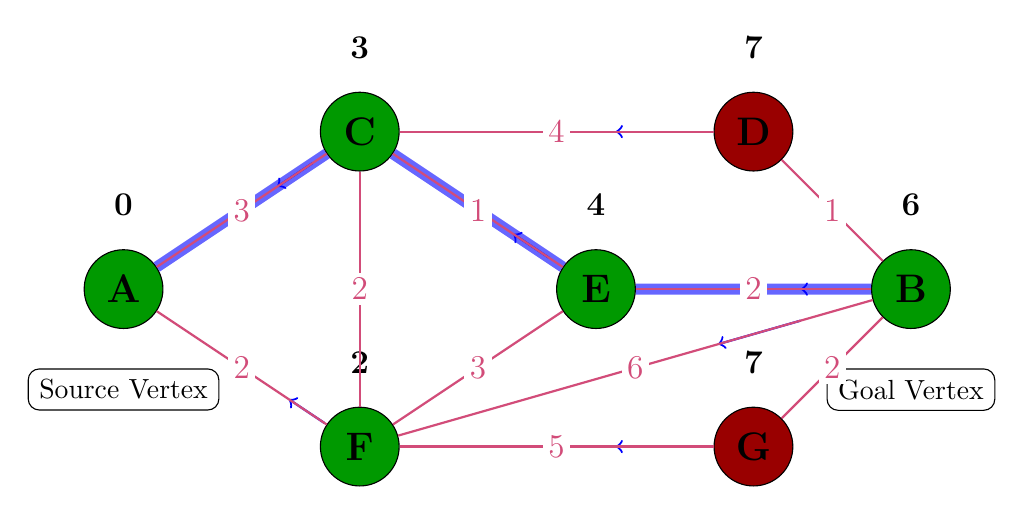
\begin{tikzpicture}[
    node distance=3cm,
    vertex/.style={circle, draw, fill=gray!70, minimum size=1cm, font=\Large\bfseries},
    edge/.style={draw, thick, color=purple!70},
    weight/.style={fill=white, inner sep=2pt, font=\large}
]

% Define node positions
\node[vertex, fill=green!60!black] (A) at (-4, 0) {A};
\node[vertex, fill=green!60!black] (C) at (-1, 2) {C};
\node[vertex, fill=green!60!black] (F) at (-1, -2) {F};
\node[vertex, fill=green!60!black] (E) at (2, 0) {E};
\node[vertex, fill=red!60!black] (D) at (4, 2) {D};
\node[vertex, fill=green!60!black] (B) at (6, 0) {B};
\node[vertex, fill=red!60!black] (G) at (4, -2) {G};

% Blue arrows for Picture 8 (pointing from child to parent)
\draw[->, blue, thick] ($ (D)!0.2!(C) $) -- ($ (D)!0.35!(C) $);
\draw[->, blue, thick] ($ (G)!0.2!(F) $) -- ($ (G)!0.35!(F) $);
\draw[->, blue, thick] ($ (C)!0.2!(A) $) -- ($ (C)!0.35!(A) $);
\draw[->, blue, thick] ($ (E)!0.2!(C) $) -- ($ (E)!0.35!(C) $);
\draw[->, blue, thick] ($ (B)!0.2!(E) $) -- ($ (B)!0.35!(E) $);
\draw[->, blue, thick] ($ (F)!0.15!(A) $) -- ($ (F)!0.3!(A) $);
\draw[->, blue, thick] ($ (B)!0.2!(F) $) -- ($ (B)!0.35!(F) $);

% Shortest path from B to A (thick partially transparent blue line)
\draw[blue, line width=4pt, opacity=0.6] (B) -- (E) -- (C) -- (A);

% Add distance labels above vertices
\node[above=0.3cm of A, font=\large\bfseries] {0};
\node[above=0.3cm of C, font=\large\bfseries] {3};
\node[above=0.3cm of F, font=\large\bfseries] {2};
\node[above=0.3cm of E, font=\large\bfseries] {4};
\node[above=0.3cm of D, font=\large\bfseries] {7};
\node[above=0.3cm of B, font=\large\bfseries] {6};
\node[above=0.3cm of G, font=\large\bfseries] {7};

% Add source vertex label
\node[below=0.5cm of A, draw, fill=white, rounded corners, inner sep=4pt] {Source Vertex};

% Add goal vertex label
\node[below=0.5cm of B, draw, fill=white, rounded corners, inner sep=4pt] {Goal Vertex};

% Draw edges with weights
\draw[edge] (A) -- (C) node[weight, midway] {3};
\draw[edge] (A) -- (F) node[weight, midway] {2};
\draw[edge] (C) -- (D) node[weight, midway] {4};
\draw[edge] (C) -- (E) node[weight, midway] {1};
\draw[edge] (C) -- (F) node[weight, midway] {2};
\draw[edge] (E) -- (F) node[weight, midway] {3};
\draw[edge] (E) -- (B) node[weight, midway] {2};
\draw[edge] (F) -- (B) node[weight, midway] {6};
\draw[edge] (D) -- (B) node[weight, midway] {1};
\draw[edge] (B) -- (G) node[weight, midway] {2};
\draw[edge] (F) -- (G) node[weight, midway] {5};

\end{tikzpicture}
\end{center}

\section{A* Algorithm}

\subsection{Overview}
A* algorithm finds the shortest path from a source vertex to a goal vertex in a weighted graph by combining the actual cost from the source with a heuristic estimate to the goal.

\subsection{Algorithm}
\textbf{Input:} A weighted directed graph $G = (V, E)$ with weight function $w: E \to \mathbb{R}_{\geq 0}$, source vertex $s \in V$, goal vertex $t \in V$, and heuristic function $h: V \to \mathbb{R}_{\geq 0}$.

\textbf{Output:} The shortest path from $s$ to $t$ and its cost.

\textbf{Initialization:}
\begin{enumerate}
    \item Set $g(s) = 0$ and $g(v) = \infty$ for all $v \in V \setminus \{s\}$
    \item Set $f(s) = g(s) + h(s) = h(s)$
    \item Create a min-priority queue $Q$ based on $f$-values and insert $(s, f(s))$
    \item Initialize parent pointers: $\pi(v) = \text{NIL}$ for all $v \in V$
\end{enumerate}

\textbf{Main Loop:}
\begin{enumerate}
    \item While $Q$ is not empty:
    \begin{enumerate}
        \item Extract $(u, f_u) = \text{ExtractMin}(Q)$
        \item If $u = t$, reconstruct path and return
        \item If $u$ has been closed, continue to next iteration
        \item Mark $u$ as closed
        \item For each neighbor $v$ of $u$ where $(u,v) \in E$:
        \begin{enumerate}
            \item Calculate tentative $g$-value: $g_{\text{new}} = g(u) + w(u,v)$
            \item If $g_{\text{new}} < g(v)$:
            \begin{itemize}
                \item Update $g(v) = g_{\text{new}}$
                \item Update $f(v) = g(v) + h(v)$
                \item Update $\pi(v) = u$
                \item Insert $(v, f(v))$ into $Q$
            \end{itemize}
        \end{enumerate}
    \end{enumerate}
\end{enumerate}

\subsection{Correctness}
A* is guaranteed to find the optimal path if the heuristic function $h$ is admissible (never overestimates the true cost) and consistent (satisfies the triangle inequality).

\subsection{Complexity}
\textbf{Time:} $O((|V| + |E|) \log |V|)$ using a binary heap\\
\textbf{Space:} $O(|V|)$

\subsection{Algorithm Requirements}
\begin{enumerate}
    \item Non-negative edge weights
    \item Admissible heuristic function ($h(v) \leq d^*(v,t)$ for all $v$)
    \item Consistent heuristic for optimal efficiency
\end{enumerate}

\subsection{Simple Example}
% PICTURE 1
\begin{center}
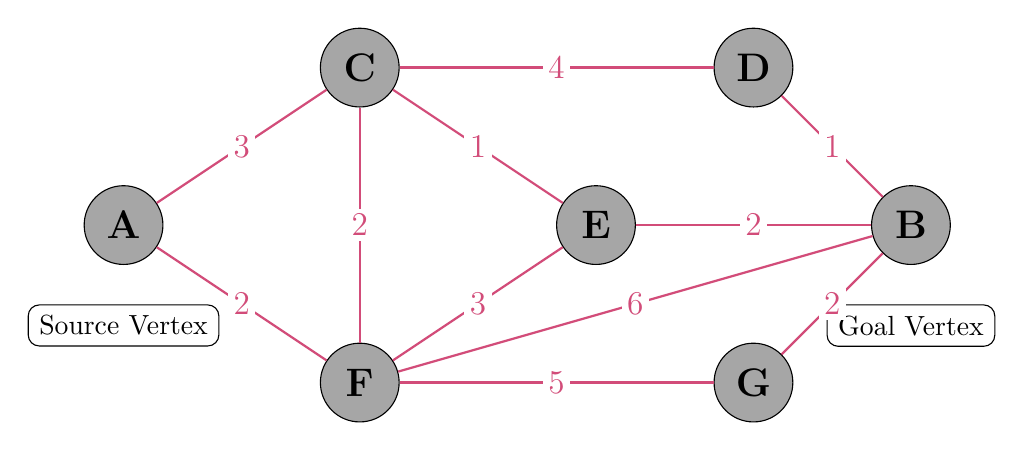
\begin{tikzpicture}[
    node distance=3cm,
    vertex/.style={circle, draw, fill=gray!70, minimum size=1cm, font=\Large\bfseries},
    edge/.style={draw, thick, color=purple!70},
    weight/.style={fill=white, inner sep=2pt, font=\large}
]

% Define node positions
\node[vertex] (A) at (-4, 0) {A};
\node[vertex] (C) at (-1, 2) {C};
\node[vertex] (F) at (-1, -2) {F};
\node[vertex] (E) at (2, 0) {E};
\node[vertex] (D) at (4, 2) {D};
\node[vertex] (B) at (6, 0) {B};
\node[vertex] (G) at (4, -2) {G};

% Add source vertex label
\node[below=0.5cm of A, draw, fill=white, rounded corners, inner sep=4pt] {Source Vertex};

% Add goal vertex label
\node[below=0.5cm of B, draw, fill=white, rounded corners, inner sep=4pt] {Goal Vertex};

% Draw edges with weights
\draw[edge] (A) -- (C) node[weight, midway] {3};
\draw[edge] (A) -- (F) node[weight, midway] {2};
\draw[edge] (C) -- (D) node[weight, midway] {4};
\draw[edge] (C) -- (E) node[weight, midway] {1};
\draw[edge] (C) -- (F) node[weight, midway] {2};
\draw[edge] (E) -- (F) node[weight, midway] {3};
\draw[edge] (E) -- (B) node[weight, midway] {2};
\draw[edge] (F) -- (B) node[weight, midway] {6};
\draw[edge] (D) -- (B) node[weight, midway] {1};
\draw[edge] (B) -- (G) node[weight, midway] {2};
\draw[edge] (F) -- (G) node[weight, midway] {5};

\end{tikzpicture}
\end{center}

% ----------- PICTURE 2 ----------
\subsection{Algorithm Initialization}
Heuristic values: $h(A)=7.2$, $h(B)=0$, $h(C)=5.4$, $h(D)=2.2$, $h(E)=3.6$, $h(F)=6.3$, $h(G)=2.8$
\begin{center}
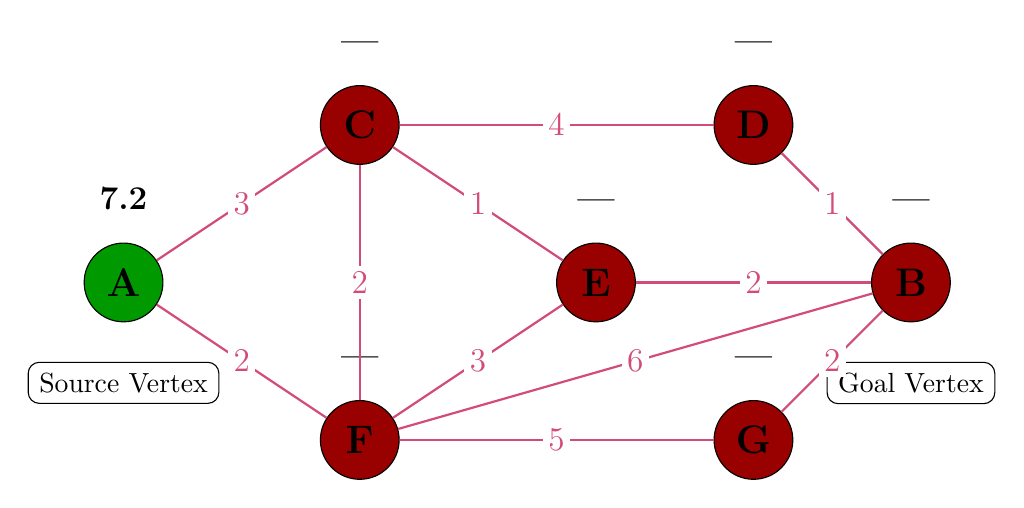
\begin{tikzpicture}[
    node distance=3cm,
    vertex/.style={circle, draw, fill=gray!70, minimum size=1cm, font=\Large\bfseries},
    edge/.style={draw, thick, color=purple!70},
    weight/.style={fill=white, inner sep=2pt, font=\large}
]

% Define node positions
\node[vertex, fill=green!60!black] (A) at (-4, 0) {A};
\node[vertex, fill=red!60!black] (C) at (-1, 2) {C};
\node[vertex, fill=red!60!black] (F) at (-1, -2) {F};
\node[vertex, fill=red!60!black] (E) at (2, 0) {E};
\node[vertex, fill=red!60!black] (D) at (4, 2) {D};
\node[vertex, fill=red!60!black] (B) at (6, 0) {B};
\node[vertex, fill=red!60!black] (G) at (4, -2) {G};

% Add f-value labels above vertices
\node[above=0.3cm of A, font=\large\bfseries] {7.2};
\node[above=0.3cm of C, font=\large\bfseries] {---};
\node[above=0.3cm of F, font=\large\bfseries] {---};
\node[above=0.3cm of E, font=\large\bfseries] {---};
\node[above=0.3cm of D, font=\large\bfseries] {---};
\node[above=0.3cm of B, font=\large\bfseries] {---};
\node[above=0.3cm of G, font=\large\bfseries] {---};

% Add source vertex label
\node[below=0.5cm of A, draw, fill=white, rounded corners, inner sep=4pt] {Source Vertex};

% Add goal vertex label
\node[below=0.5cm of B, draw, fill=white, rounded corners, inner sep=4pt] {Goal Vertex};

% Draw edges with weights
\draw[edge] (A) -- (C) node[weight, midway] {3};
\draw[edge] (A) -- (F) node[weight, midway] {2};
\draw[edge] (C) -- (D) node[weight, midway] {4};
\draw[edge] (C) -- (E) node[weight, midway] {1};
\draw[edge] (C) -- (F) node[weight, midway] {2};
\draw[edge] (E) -- (F) node[weight, midway] {3};
\draw[edge] (E) -- (B) node[weight, midway] {2};
\draw[edge] (F) -- (B) node[weight, midway] {6};
\draw[edge] (D) -- (B) node[weight, midway] {1};
\draw[edge] (B) -- (G) node[weight, midway] {2};
\draw[edge] (F) -- (G) node[weight, midway] {5};

\end{tikzpicture}
\end{center}

% ----------- PICTURE 3 ----------
\subsection{Processing Source Vertex A}
\begin{center}
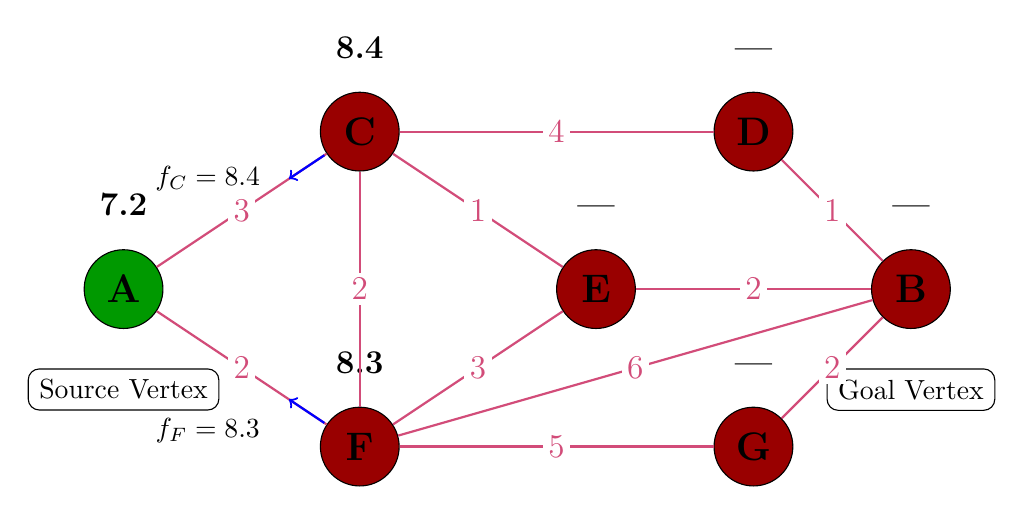
\begin{tikzpicture}[
    node distance=3cm,
    vertex/.style={circle, draw, fill=gray!70, minimum size=1cm, font=\Large\bfseries},
    edge/.style={draw, thick, color=purple!70},
    weight/.style={fill=white, inner sep=2pt, font=\large}
]

% Define node positions
\node[vertex, fill=green!60!black] (A) at (-4, 0) {A};
\node[vertex, fill=red!60!black] (C) at (-1, 2) {C};
\node[vertex, fill=red!60!black] (F) at (-1, -2) {F};
\node[vertex, fill=red!60!black] (E) at (2, 0) {E};
\node[vertex, fill=red!60!black] (D) at (4, 2) {D};
\node[vertex, fill=red!60!black] (B) at (6, 0) {B};
\node[vertex, fill=red!60!black] (G) at (4, -2) {G};

% Add f-value labels above vertices
\node[above=0.3cm of A, font=\large\bfseries] {7.2};
\node[above=0.3cm of C, font=\large\bfseries] {8.4};
\node[above=0.3cm of F, font=\large\bfseries] {8.3};
\node[above=0.3cm of E, font=\large\bfseries] {---};
\node[above=0.3cm of D, font=\large\bfseries] {---};
\node[above=0.3cm of B, font=\large\bfseries] {---};
\node[above=0.3cm of G, font=\large\bfseries] {---};

% Add source vertex label
\node[below=0.5cm of A, draw, fill=white, rounded corners, inner sep=4pt] {Source Vertex};

% Add goal vertex label
\node[below=0.5cm of B, draw, fill=white, rounded corners, inner sep=4pt] {Goal Vertex};

% Draw edges with weights
\draw[edge] (A) -- (C) node[weight, midway] {3} node[pos=0.3, above=4mm, color=black] {$f_C = 8.4$};
\draw[edge] (A) -- (F) node[weight, midway] {2} node[pos=0.3, below=8mm, color=black] {$f_F = 8.3$};
\draw[edge] (C) -- (D) node[weight, midway] {4};
\draw[edge] (C) -- (E) node[weight, midway] {1};
\draw[edge] (C) -- (F) node[weight, midway] {2};
\draw[edge] (E) -- (F) node[weight, midway] {3};
\draw[edge] (E) -- (B) node[weight, midway] {2};
\draw[edge] (F) -- (B) node[weight, midway] {6};
\draw[edge] (D) -- (B) node[weight, midway] {1};
\draw[edge] (B) -- (G) node[weight, midway] {2};
\draw[edge] (F) -- (G) node[weight, midway] {5};

% Blue arrows for Picture 3 (pointing from child to parent)
\draw[->, blue, thick] ($ (C)!0.15!(A) $) -- ($ (C)!0.3!(A) $);
\draw[->, blue, thick] ($ (F)!0.15!(A) $) -- ($ (F)!0.3!(A) $);

\end{tikzpicture}
\end{center}

% ----------- PICTURE 4 ----------
\subsection{Processing Vertex F}
\begin{center}
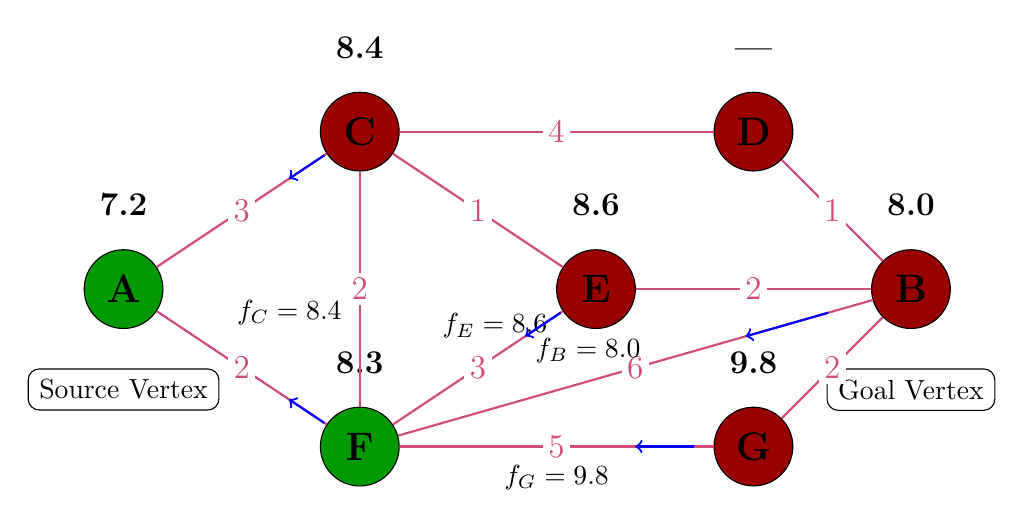
\begin{tikzpicture}[
    node distance=3cm,
    vertex/.style={circle, draw, fill=gray!70, minimum size=1cm, font=\Large\bfseries},
    edge/.style={draw, thick, color=purple!70},
    weight/.style={fill=white, inner sep=2pt, font=\large}
]

% Define node positions
\node[vertex, fill=green!60!black] (A) at (-4, 0) {A};
\node[vertex, fill=red!60!black] (C) at (-1, 2) {C};
\node[vertex, fill=green!60!black] (F) at (-1, -2) {F};
\node[vertex, fill=red!60!black] (E) at (2, 0) {E};
\node[vertex, fill=red!60!black] (D) at (4, 2) {D};
\node[vertex, fill=red!60!black] (B) at (6, 0) {B};
\node[vertex, fill=red!60!black] (G) at (4, -2) {G};

% Add f-value labels above vertices
\node[above=0.3cm of A, font=\large\bfseries] {7.2};
\node[above=0.3cm of C, font=\large\bfseries] {8.4};
\node[above=0.3cm of F, font=\large\bfseries] {8.3};
\node[above=0.3cm of E, font=\large\bfseries] {8.6};
\node[above=0.3cm of D, font=\large\bfseries] {---};
\node[above=0.3cm of B, font=\large\bfseries] {8.0};
\node[above=0.3cm of G, font=\large\bfseries] {9.8};

% Add source vertex label
\node[below=0.5cm of A, draw, fill=white, rounded corners, inner sep=4pt] {Source Vertex};

% Add goal vertex label
\node[below=0.5cm of B, draw, fill=white, rounded corners, inner sep=4pt] {Goal Vertex};

% Draw edges with weights and f-value calculations
\draw[edge] (A) -- (C) node[weight, midway] {3};
\draw[edge] (A) -- (F) node[weight, midway] {2};
\draw[edge] (C) -- (D) node[weight, midway] {4};
\draw[edge] (C) -- (E) node[weight, midway] {1};
\draw[edge] (C) -- (F) node[weight, midway] {2} node[pos=0.6, left=1mm, color=black] {$f_C = 8.4$};
\draw[edge] (E) -- (F) node[weight, midway] {3} node[pos=0.4, above=1mm, color=black] {$f_E = 8.6$};
\draw[edge] (E) -- (B) node[weight, midway] {2};
\draw[edge] (F) -- (B) node[weight, midway] {6} node[pos=0.4, above=1mm, color=black] {$f_B = 8.0$};
\draw[edge] (D) -- (B) node[weight, midway] {1};
\draw[edge] (B) -- (G) node[weight, midway] {2};
\draw[edge] (F) -- (G) node[weight, midway] {5} node[pos=0.5, below=1mm, color=black] {$f_G = 9.8$};

% Blue arrows for Picture 4 (pointing from child to parent)
\draw[->, blue, thick] ($ (E)!0.15!(F) $) -- ($ (E)!0.3!(F) $);
\draw[->, blue, thick] ($ (B)!0.15!(F) $) -- ($ (B)!0.3!(F) $);
\draw[->, blue, thick] ($ (G)!0.15!(F) $) -- ($ (G)!0.3!(F) $);
\draw[->, blue, thick] ($ (C)!0.15!(A) $) -- ($ (C)!0.3!(A) $);
\draw[->, blue, thick] ($ (F)!0.15!(A) $) -- ($ (F)!0.3!(A) $);

\end{tikzpicture}
\end{center}

% ----------- PICTURE 5 ----------
\subsection{Processing Vertex B (First Time)}
Note: B is found but algorithm continues to ensure optimality
\begin{center}
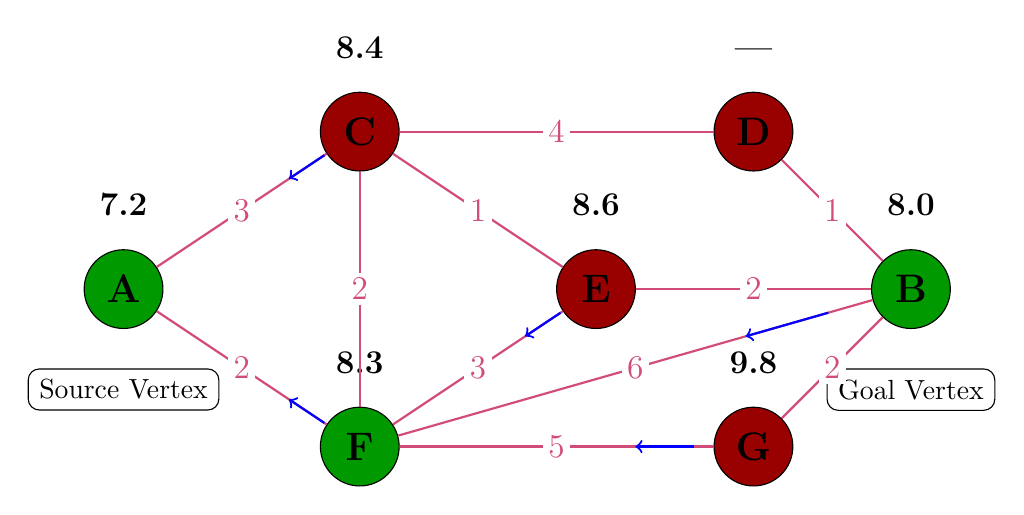
\begin{tikzpicture}[
    node distance=3cm,
    vertex/.style={circle, draw, fill=gray!70, minimum size=1cm, font=\Large\bfseries},
    edge/.style={draw, thick, color=purple!70},
    weight/.style={fill=white, inner sep=2pt, font=\large}
]

% Define node positions
\node[vertex, fill=green!60!black] (A) at (-4, 0) {A};
\node[vertex, fill=red!60!black] (C) at (-1, 2) {C};
\node[vertex, fill=green!60!black] (F) at (-1, -2) {F};
\node[vertex, fill=red!60!black] (E) at (2, 0) {E};
\node[vertex, fill=red!60!black] (D) at (4, 2) {D};
\node[vertex, fill=green!60!black] (B) at (6, 0) {B};
\node[vertex, fill=red!60!black] (G) at (4, -2) {G};

% Add f-value labels above vertices
\node[above=0.3cm of A, font=\large\bfseries] {7.2};
\node[above=0.3cm of C, font=\large\bfseries] {8.4};
\node[above=0.3cm of F, font=\large\bfseries] {8.3};
\node[above=0.3cm of E, font=\large\bfseries] {8.6};
\node[above=0.3cm of D, font=\large\bfseries] {---};
\node[above=0.3cm of B, font=\large\bfseries] {8.0};
\node[above=0.3cm of G, font=\large\bfseries] {9.8};

% Add source vertex label
\node[below=0.5cm of A, draw, fill=white, rounded corners, inner sep=4pt] {Source Vertex};

% Add goal vertex label
\node[below=0.5cm of B, draw, fill=white, rounded corners, inner sep=4pt] {Goal Vertex};

% Draw edges with weights
\draw[edge] (A) -- (C) node[weight, midway] {3};
\draw[edge] (A) -- (F) node[weight, midway] {2};
\draw[edge] (C) -- (D) node[weight, midway] {4};
\draw[edge] (C) -- (E) node[weight, midway] {1};
\draw[edge] (C) -- (F) node[weight, midway] {2};
\draw[edge] (E) -- (F) node[weight, midway] {3};
\draw[edge] (E) -- (B) node[weight, midway] {2};
\draw[edge] (F) -- (B) node[weight, midway] {6};
\draw[edge] (D) -- (B) node[weight, midway] {1};
\draw[edge] (B) -- (G) node[weight, midway] {2};
\draw[edge] (F) -- (G) node[weight, midway] {5};

% Blue arrows (same as before)
\draw[->, blue, thick] ($ (E)!0.15!(F) $) -- ($ (E)!0.3!(F) $);
\draw[->, blue, thick] ($ (B)!0.15!(F) $) -- ($ (B)!0.3!(F) $);
\draw[->, blue, thick] ($ (G)!0.15!(F) $) -- ($ (G)!0.3!(F) $);
\draw[->, blue, thick] ($ (C)!0.15!(A) $) -- ($ (C)!0.3!(A) $);
\draw[->, blue, thick] ($ (F)!0.15!(A) $) -- ($ (F)!0.3!(A) $);

\end{tikzpicture}
\end{center}

% ----------- PICTURE 6 ----------
\subsection{Processing Vertex C}
\begin{center}
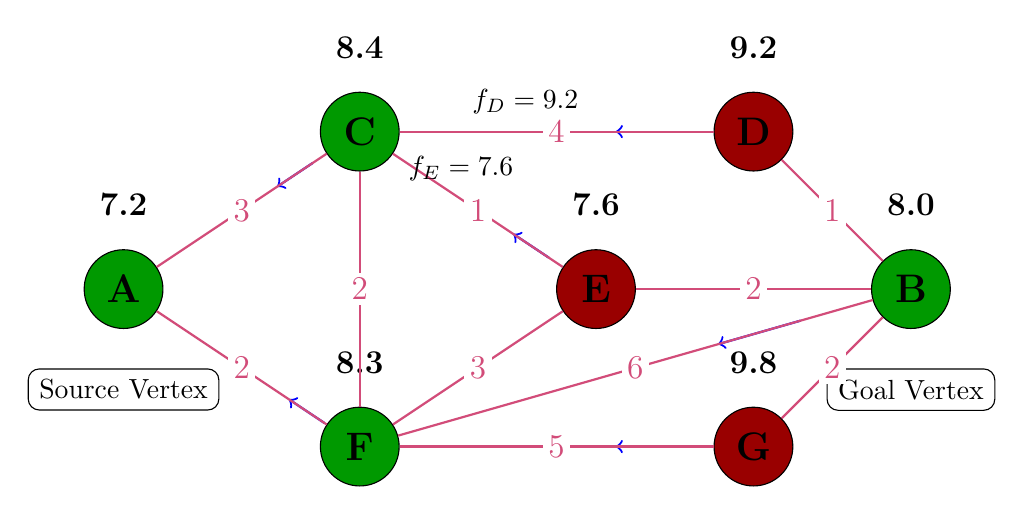
\begin{tikzpicture}[
    node distance=3cm,
    vertex/.style={circle, draw, fill=gray!70, minimum size=1cm, font=\Large\bfseries},
    edge/.style={draw, thick, color=purple!70},
    weight/.style={fill=white, inner sep=2pt, font=\large}
]

% Define node positions
\node[vertex, fill=green!60!black] (A) at (-4, 0) {A};
\node[vertex, fill=green!60!black] (C) at (-1, 2) {C};
\node[vertex, fill=green!60!black] (F) at (-1, -2) {F};
\node[vertex, fill=red!60!black] (E) at (2, 0) {E};
\node[vertex, fill=red!60!black] (D) at (4, 2) {D};
\node[vertex, fill=green!60!black] (B) at (6, 0) {B};
\node[vertex, fill=red!60!black] (G) at (4, -2) {G};

% Blue arrows for Picture 6 (pointing from child to parent)
\draw[->, blue, thick] ($ (D)!0.2!(C) $) -- ($ (D)!0.35!(C) $);
\draw[->, blue, thick] ($ (E)!0.2!(C) $) -- ($ (E)!0.35!(C) $);
\draw[->, blue, thick] ($ (B)!0.2!(F) $) -- ($ (B)!0.35!(F) $);
\draw[->, blue, thick] ($ (G)!0.2!(F) $) -- ($ (G)!0.35!(F) $);
\draw[->, blue, thick] ($ (C)!0.2!(A) $) -- ($ (C)!0.35!(A) $);
\draw[->, blue, thick] ($ (F)!0.15!(A) $) -- ($ (F)!0.3!(A) $);

% Add f-value labels above vertices
\node[above=0.3cm of A, font=\large\bfseries] {7.2};
\node[above=0.3cm of C, font=\large\bfseries] {8.4};
\node[above=0.3cm of F, font=\large\bfseries] {8.3};
\node[above=0.3cm of E, font=\large\bfseries] {7.6};
\node[above=0.3cm of D, font=\large\bfseries] {9.2};
\node[above=0.3cm of B, font=\large\bfseries] {8.0};
\node[above=0.3cm of G, font=\large\bfseries] {9.8};

% Add source vertex label
\node[below=0.5cm of A, draw, fill=white, rounded corners, inner sep=4pt] {Source Vertex};

% Add goal vertex label
\node[below=0.5cm of B, draw, fill=white, rounded corners, inner sep=4pt] {Goal Vertex};

% Draw edges with weights and f-value calculations
\draw[edge] (A) -- (C) node[weight, midway] {3};
\draw[edge] (A) -- (F) node[weight, midway] {2};
\draw[edge] (C) -- (D) node[weight, midway] {4} node[pos=0.4, above=1mm, color=black] {$f_D = 9.2$};
\draw[edge] (C) -- (E) node[weight, midway] {1} node[pos=0.4, above=1mm, color=black] {$f_E = 7.6$};
\draw[edge] (C) -- (F) node[weight, midway] {2};
\draw[edge] (E) -- (F) node[weight, midway] {3};
\draw[edge] (E) -- (B) node[weight, midway] {2};
\draw[edge] (F) -- (B) node[weight, midway] {6};
\draw[edge] (D) -- (B) node[weight, midway] {1};
\draw[edge] (B) -- (G) node[weight, midway] {2};
\draw[edge] (F) -- (G) node[weight, midway] {5};

\end{tikzpicture}
\end{center}

% ----------- PICTURE 7 ----------
\subsection{Processing Vertex E}
\begin{center}
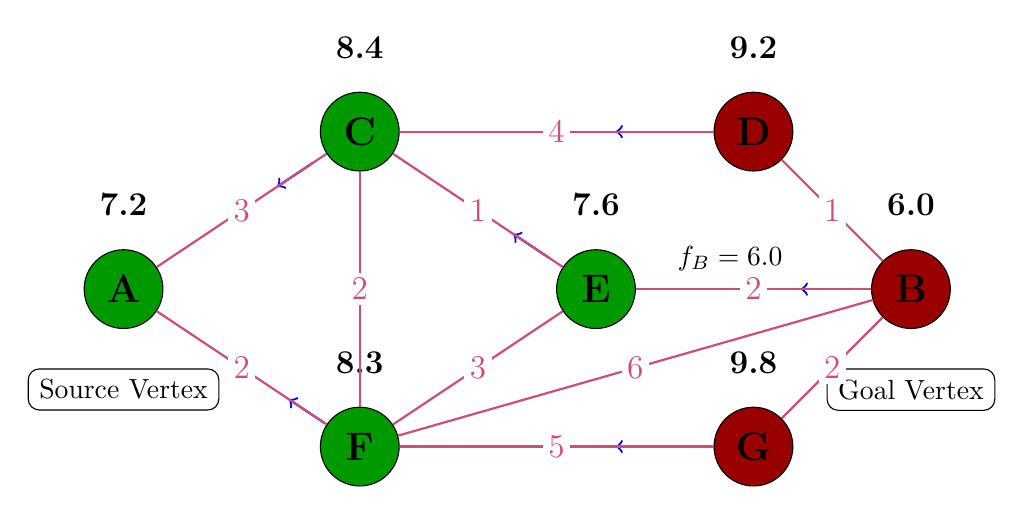
\begin{tikzpicture}[
    node distance=3cm,
    vertex/.style={circle, draw, fill=gray!70, minimum size=1cm, font=\Large\bfseries},
    edge/.style={draw, thick, color=purple!70},
    weight/.style={fill=white, inner sep=2pt, font=\large}
]

% Define node positions
\node[vertex, fill=green!60!black] (A) at (-4, 0) {A};
\node[vertex, fill=green!60!black] (C) at (-1, 2) {C};
\node[vertex, fill=green!60!black] (F) at (-1, -2) {F};
\node[vertex, fill=green!60!black] (E) at (2, 0) {E};
\node[vertex, fill=red!60!black] (D) at (4, 2) {D};
\node[vertex, fill=red!60!black] (B) at (6, 0) {B};
\node[vertex, fill=red!60!black] (G) at (4, -2) {G};

% Blue arrows for Picture 7 (pointing from child to parent)
\draw[->, blue, thick] ($ (D)!0.2!(C) $) -- ($ (D)!0.35!(C) $);
\draw[->, blue, thick] ($ (B)!0.2!(E) $) -- ($ (B)!0.35!(E) $);
\draw[->, blue, thick] ($ (G)!0.2!(F) $) -- ($ (G)!0.35!(F) $);
\draw[->, blue, thick] ($ (C)!0.2!(A) $) -- ($ (C)!0.35!(A) $);
\draw[->, blue, thick] ($ (E)!0.2!(C) $) -- ($ (E)!0.35!(C) $);
\draw[->, blue, thick] ($ (F)!0.15!(A) $) -- ($ (F)!0.3!(A) $);

% Add f-value labels above vertices
\node[above=0.3cm of A, font=\large\bfseries] {7.2};
\node[above=0.3cm of C, font=\large\bfseries] {8.4};
\node[above=0.3cm of F, font=\large\bfseries] {8.3};
\node[above=0.3cm of E, font=\large\bfseries] {7.6};
\node[above=0.3cm of D, font=\large\bfseries] {9.2};
\node[above=0.3cm of B, font=\large\bfseries] {6.0};
\node[above=0.3cm of G, font=\large\bfseries] {9.8};

% Add source vertex label
\node[below=0.5cm of A, draw, fill=white, rounded corners, inner sep=4pt] {Source Vertex};

% Add goal vertex label
\node[below=0.5cm of B, draw, fill=white, rounded corners, inner sep=4pt] {Goal Vertex};

% Draw edges with weights and f-value calculations
\draw[edge] (A) -- (C) node[weight, midway] {3};
\draw[edge] (A) -- (F) node[weight, midway] {2};
\draw[edge] (C) -- (D) node[weight, midway] {4};
\draw[edge] (C) -- (E) node[weight, midway] {1};
\draw[edge] (C) -- (F) node[weight, midway] {2};
\draw[edge] (E) -- (F) node[weight, midway] {3};
\draw[edge] (E) -- (B) node[weight, midway] {2} node[pos=0.4, above=1mm, color=black] {$f_B = 6.0$};
\draw[edge] (F) -- (B) node[weight, midway] {6};
\draw[edge] (D) -- (B) node[weight, midway] {1};
\draw[edge] (B) -- (G) node[weight, midway] {2};
\draw[edge] (F) -- (G) node[weight, midway] {5};

\end{tikzpicture}
\end{center}

% ----------- PICTURE 8 ----------
\subsection{Processing Vertex B (Second Time - Optimal)}
\begin{center}
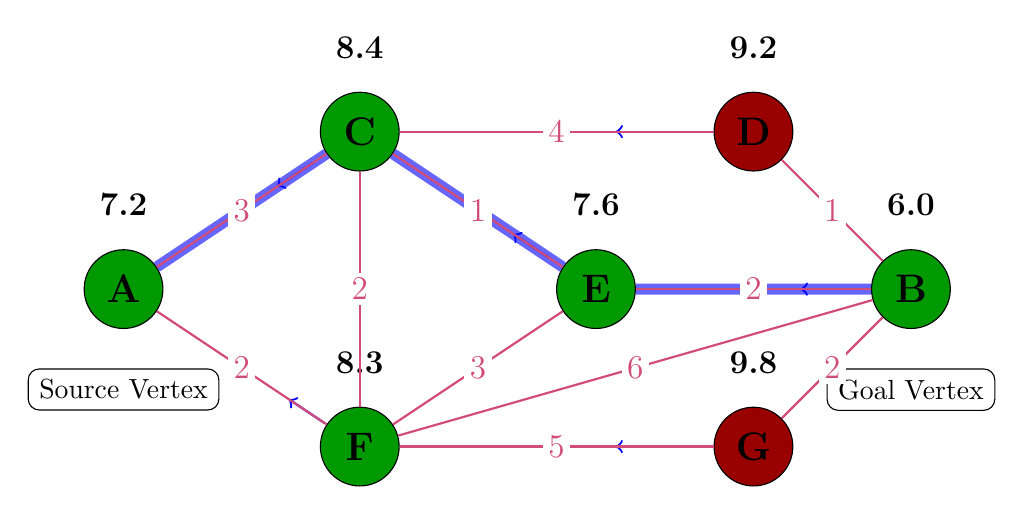
\begin{tikzpicture}[
    node distance=3cm,
    vertex/.style={circle, draw, fill=gray!70, minimum size=1cm, font=\Large\bfseries},
    edge/.style={draw, thick, color=purple!70},
    weight/.style={fill=white, inner sep=2pt, font=\large}
]

% Define node positions
\node[vertex, fill=green!60!black] (A) at (-4, 0) {A};
\node[vertex, fill=green!60!black] (C) at (-1, 2) {C};
\node[vertex, fill=green!60!black] (F) at (-1, -2) {F};
\node[vertex, fill=green!60!black] (E) at (2, 0) {E};
\node[vertex, fill=red!60!black] (D) at (4, 2) {D};
\node[vertex, fill=green!60!black] (B) at (6, 0) {B};
\node[vertex, fill=red!60!black] (G) at (4, -2) {G};

% Blue arrows for Picture 8 (pointing from child to parent)
\draw[->, blue, thick] ($ (D)!0.2!(C) $) -- ($ (D)!0.35!(C) $);
\draw[->, blue, thick] ($ (B)!0.2!(E) $) -- ($ (B)!0.35!(E) $);
\draw[->, blue, thick] ($ (G)!0.2!(F) $) -- ($ (G)!0.35!(F) $);
\draw[->, blue, thick] ($ (C)!0.2!(A) $) -- ($ (C)!0.35!(A) $);
\draw[->, blue, thick] ($ (E)!0.2!(C) $) -- ($ (E)!0.35!(C) $);
\draw[->, blue, thick] ($ (F)!0.15!(A) $) -- ($ (F)!0.3!(A) $);

% Shortest path from A to B (thick partially transparent blue line)
\draw[blue, line width=4pt, opacity=0.6] (A) -- (C) -- (E) -- (B);

% Add f-value labels above vertices
\node[above=0.3cm of A, font=\large\bfseries] {7.2};
\node[above=0.3cm of C, font=\large\bfseries] {8.4};
\node[above=0.3cm of F, font=\large\bfseries] {8.3};
\node[above=0.3cm of E, font=\large\bfseries] {7.6};
\node[above=0.3cm of D, font=\large\bfseries] {9.2};
\node[above=0.3cm of B, font=\large\bfseries] {6.0};
\node[above=0.3cm of G, font=\large\bfseries] {9.8};

% Add source vertex label
\node[below=0.5cm of A, draw, fill=white, rounded corners, inner sep=4pt] {Source Vertex};

% Add goal vertex label
\node[below=0.5cm of B, draw, fill=white, rounded corners, inner sep=4pt] {Goal Vertex};

% Draw edges with weights
\draw[edge] (A) -- (C) node[weight, midway] {3};
\draw[edge] (A) -- (F) node[weight, midway] {2};
\draw[edge] (C) -- (D) node[weight, midway] {4};
\draw[edge] (C) -- (E) node[weight, midway] {1};
\draw[edge] (C) -- (F) node[weight, midway] {2};
\draw[edge] (E) -- (F) node[weight, midway] {3};
\draw[edge] (E) -- (B) node[weight, midway] {2};
\draw[edge] (F) -- (B) node[weight, midway] {6};
\draw[edge] (D) -- (B) node[weight, midway] {1};
\draw[edge] (B) -- (G) node[weight, midway] {2};
\draw[edge] (F) -- (G) node[weight, midway] {5};

\end{tikzpicture}
\end{center}

\subsection{Shortest Path from A to B}
The A* algorithm found the optimal path: A → C → E → B with total cost 6.

Key insight: Even though B was first discovered via F with f=8.0, the algorithm continued and found a better path through C and E with f=6.0. This demonstrates why A* must continue until the goal is extracted from the priority queue with the minimum f-value.

\end{document}